\documentclass{standalone}

\usepackage{tikz}
\usetikzlibrary{colorbrewer, decorations.pathreplacing}

\begin{document}
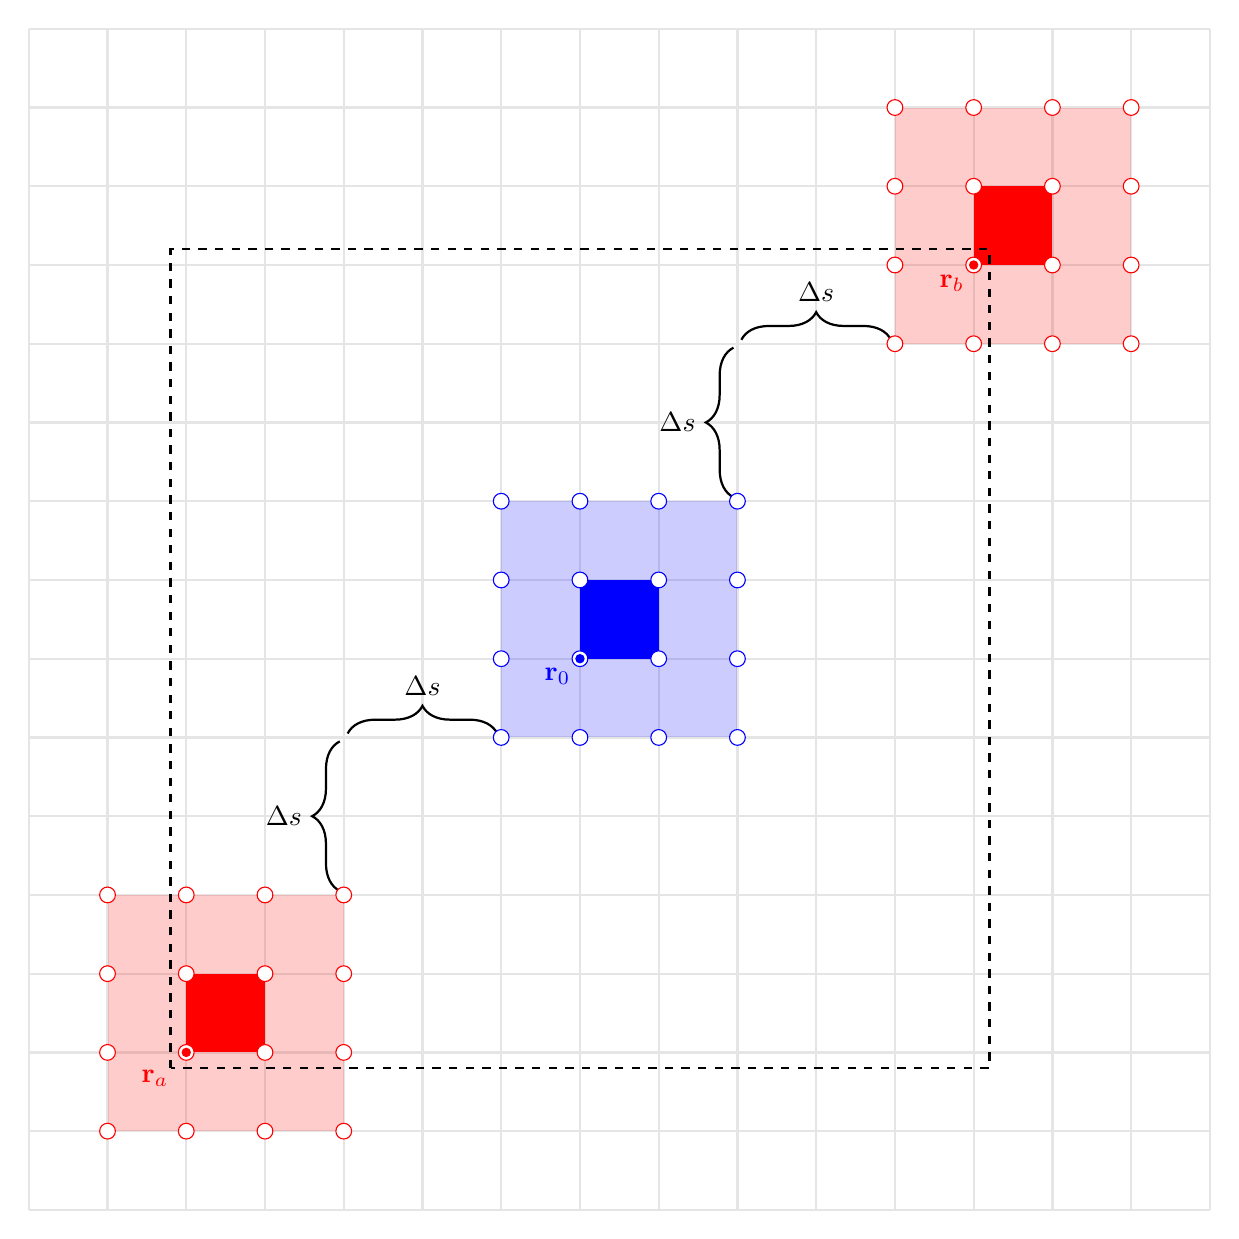
\begin{tikzpicture}

\draw[step=1, black, thick, opacity=0.1] (-7,-7) grid (8, 8);

\draw[thick, decorate,decoration={brace,amplitude=10}] (-2.95,-0.95) -- (-1.05, -0.95) node [midway, above, yshift=10] {$\Delta s$};
\draw[thick, decorate,decoration={brace,amplitude=10}] (-3.05,-2.95) -- (-3.05, -1.05) node [midway, anchor=east, xshift=-10] {$\Delta s$};

\draw[thick, decorate,decoration={brace,amplitude=10}] (1.95,2.05) -- (1.95,3.95) node [midway, anchor=east, xshift=-10] {$\Delta s$};
\draw[thick, decorate,decoration={brace,amplitude=10}] (2.05,4.05) -- (3.95,4.05) node [midway, anchor=south, yshift=10] {$\Delta s$};



\fill[blue] (0,0) rectangle (1, 1);
\fill[blue, opacity=0.2] (-1,-1) rectangle (2, 2);

\foreach \x in {-1,...,2} {
  \foreach \y in {-1,...,2} {

    \draw[blue, fill=white, radius=0.1] (\x,\y) circle;

  }
}
\fill[blue, radius=0.06] node[anchor=north east] (0, 0) {$\mathbf{r}_0$} circle;




\fill[red] (-5,-5) rectangle (-4, -4);
\fill[red, opacity=0.2] (-6,-6) rectangle (-3, -3);

\foreach \x in {-6,-5,...,-3} {
  \foreach \y in {-6, -5, ..., -3} {
    \draw[red, fill=white, radius=0.1] (\x, \y) circle;
  }
}
\fill[red, radius=0.06] (-5, -5) node[anchor=north east, xshift=-3, yshift=-3] {$\mathbf{r}_a$} circle;




\fill[red] (5,5) rectangle (6, 6);
\fill[red, opacity=0.2] (4, 4) rectangle (7, 7);

\foreach \x in {4,...,7} {
  \foreach \y in {4,...,7} {
    \draw[red, fill=white, radius=0.1] (\x, \y) circle;
  }
}
\fill[red, radius=0.06] (5, 5) node[anchor=north east] {$\mathbf{r}_b$} circle;


\draw[thick, dashed] (-5.2,-5.2) rectangle (5.2, 5.2);

\end{tikzpicture}
\end{document}
